% Template for Cogsci submission with R Markdown

% Stuff changed from original Markdown PLOS Template
\documentclass[10pt, letterpaper]{article}

\usepackage{cogsci}
\usepackage{pslatex}
\usepackage{float}
\usepackage{caption}

% amsmath package, useful for mathematical formulas
\usepackage{amsmath}

% amssymb package, useful for mathematical symbols
\usepackage{amssymb}

% hyperref package, useful for hyperlinks
\usepackage{hyperref}

% graphicx package, useful for including eps and pdf graphics
% include graphics with the command \includegraphics
\usepackage{graphicx}

% Sweave(-like)
\usepackage{fancyvrb}
\DefineVerbatimEnvironment{Sinput}{Verbatim}{fontshape=sl}
\DefineVerbatimEnvironment{Soutput}{Verbatim}{}
\DefineVerbatimEnvironment{Scode}{Verbatim}{fontshape=sl}
\newenvironment{Schunk}{}{}
\DefineVerbatimEnvironment{Code}{Verbatim}{}
\DefineVerbatimEnvironment{CodeInput}{Verbatim}{fontshape=sl}
\DefineVerbatimEnvironment{CodeOutput}{Verbatim}{}
\newenvironment{CodeChunk}{}{}

% cite package, to clean up citations in the main text. Do not remove.
\usepackage{cite}

\usepackage{color}

% Use doublespacing - comment out for single spacing
%\usepackage{setspace}
%\doublespacing


% % Text layout
% \topmargin 0.0cm
% \oddsidemargin 0.5cm
% \evensidemargin 0.5cm
% \textwidth 16cm
% \textheight 21cm

\title{The Semantics and Pragmatics of Logical Connectives: Adults' and
Children's Interpretations of \emph{and} and \emph{or} in a Guessing
Game}


\author{{\large \bf Masoud Jasbi} \\ \texttt{masoudj@stanford.edu} \\ Department of Linguistics \\ Stanford University \And {\large \bf Michael C. Frank} \\ \texttt{mcfrank@stanford.edu} \\ Department of Psychology \\ Stanford University}

\begin{document}

\maketitle

\begin{abstract}
Logical connectives \emph{and} and \emph{or} have been a source of
insight into the roles of semantics and pragmatics in children's
linguistic development. Previous research has suggested that adults and
children may differ in their interpretation of \emph{or} in two ways.
First, unlike adults, children may interpret \emph{or} as \emph{and}
(Tieu et al., 2016). Second, children interpret \emph{or} as inclusive
disjunction while adults interpret it as exclusive disjunction
(Chierchia, Crain, Guasti, Gualmini, \& Meroni, 2001; Crain, 2012, among
others). We report the results of two experimental studies with truth
value judgement tasks that agree with the latter but not the former
claim. The results suggest that children do not interpret \emph{or} as
\emph{and} but they do interpret it as inclusive disjunction more often
than adults. We discuss our analysis of children's linguistic feedback
in the experiment that suggests the difference in inclusive
interpreation may be caused by truth value judgement tasks rather than
differences between children and adults in pragmatic competence.

\textbf{Keywords:}
semantics; pragmatics; disjunction; conjunction; language development.
\end{abstract}

\section{Introduction}\label{introduction}

An airport sign reads ``\emph{If you see something, say something.}''
Taken literally, this is a trivial request, but readers infer an
interpretation that goes far beyond the literal meanings of the words.
How much of what we interpret is due to literal meaning (semantics) and
how much due to our general-purpose inferential abilities (pragmatics)?
In this paper, we address this question by investigating adult and
children's interpretation of logical words \emph{and} and \emph{or}.

Despite their simple appearance, \emph{and} and \emph{or} have been a
major source of insight into the contributions of semantics and
pragmatics to language interpretation. The meaning of \emph{and} has
always been unambiguously associaated with logical conjunction. A
conjunction is true when each individual conjunct is true. The meaning
of \emph{or}, however, has proven hard to capture. It has two possible
interpretations: \textbf{inclusive} or logical disjunction and
\textbf{exclusive} disjunction. An \textbf{inclusive} disjunction is
true when either disjunct or both are true. On the other hand, an
exclusive disjunction is true when only one of the disjuncts is true --
not both. Until Grice (1975), it was generally assumed that \emph{or} is
ambiguous between an inclusive meaning and an exclusive one.

Grice (1975) argued against this ambiguity account. He maintained that
the core meaning of \emph{or} is inclusive disjunction. The exclusive
interpretation of it is derived from the inclusive meaning via pragmatic
reasoning. For example, ``\emph{there is a cat or a dog in the
picture}'' implies that not both animals are in the picture. This is
called the \emph{exclusivity implicature}. Grice argued that this
implicature is derived via reasoning on what the speaker of the sentence
could have said. If the speaker meant to communicate that both animals
are in the picture, s/he could have used the connective \emph{and}. He
chose \emph{or} instead, so he did not mean to communicate that both
animals are in the picture. In the Gricean account, the exclusivity
implicature is not part of \emph{or}'s meaning, but rather the result of
our reasoning on why the speaker chose \emph{or} instead of \emph{and}.

Before the emergence of this Gricean account, research on children's
interpretation of \emph{and} and \emph{or} adopted the ambiguity account
within a Piagetian framework. It was assumed that the concept of choice
between two options - in other words the exclusive meaning - is more
primitive than the so called logical inclusive meaning. It was predicted
that children start by interpreting \emph{or} as exclusive and later
learn to interpret it as inclusive disjunction. This developmental
hypothesis found initial empirical support from some experimental
studies such as Johansson \& Sjolin (1975) and Braine \& Rumain (1981).

The advent of Gricean pragmatics changed the landscape of research on
children's development of \emph{and} and \emph{or} interpretations. The
focus shifted to the differences between adults and children in semantic
vs.~pragmatic aspects of interpretation. In a series of influential
studies, Stephen Crain and his colleagues argued that unlike adults who
have an implicature-rich exclusive interpretation of \emph{or}, children
as young as three years old, interpret the meaning of \emph{or} in its
logical and inclusive sense. (Chierchia et al., 2001; Crain, 2008, 2012;
Notley, Zhou, Jensen, \& Crain, 2012) They argued that children develop
the semantics of \emph{or} before its pragmatics: they interpret
\emph{or} as inclusive disjunction but fail to enrich it with the
exclusivity implicature the way adults do. Therefore, the main
difference between children and adults is that children interpret
\emph{or} as inclusive, but adults interpret it as exclusive.

Recent investigations have added a new level of complexity to this line
of research. Tieu et al. (2016) and Singh et al. (2016) argued that a
substantial number of children in their studies (30-40\% of the samples)
interpreted \emph{or} like a conjunction. In other words, these children
do not differentiate between \emph{and} and \emph{or}. Based on previous
studies that show children undertsand the meaning of \emph{or}, they
argue that this conjunctive interpretation of \emph{or} is due to a
non-adult-like pragmatic reasoning. Children interpret \emph{A or B} as
\emph{A or B, but not only A and no only B}, resulting in \emph{A and
B}.

The current paper seeks to fill two gaps in the current literature.
First, for theoretical reasons, previous research has focused on
children's interpretation of \emph{and} and \emph{or} in complex
sentences -- for example with with other logical words such as
quantifiers \emph{every} and \emph{none}. In this paper we test children
and adults' understanding of \emph{and} and \emph{or} in simple
existential sentences like ``\emph{There is a cat or a dog}.'' Second,
previous research has tested children and adults using the binary truth
value judgement task (Crain \& Thornton, 1998). In such tasks
participants are asked whether a puppet's statement is right or wrong.
In this study, we allow participants to make use of three options:
wrong, kinda right, and right. Katsos \& Bishop (2011) showed that
ternary judgment tasks are better suited for assessing children's
pragmatic competence.

In this paper we address two main questions. First, do children (and
adults) interpret \emph{or} similar to \emph{and}? Second, do they
understand \emph{or} as inclusive disjunction, or exclusive disjunction?
We conduct two experiments to answer these questions. Experiment 1 tests
the adults' performance and sets the benchmark for children's
perfomrance in the task. Experiment 2 investigates children's
interpretaitons. The results of our experiments suggest that the answer
to the first question is \textbf{no} for both adults and children. For
the second question, the results suggest that adults are more inclined
to interpret \emph{or} as exclusive than inclusive. On the other hand,
children show judgements compatible with inclusive disjunction. We bring
an analysis of children's linguistic feedback that hints at exclusive
interpretations not captured by the truth value judgement task. We
discuss this methodological concern and possible ways of addressing it.

\section{Experiment 1}\label{experiment-1}

The goal of this study was to examin adults' interpretation of the
connectives \emph{and} and \emph{or} as a benchmark for children's
interpretations. We designed the study as a card game in which
participants saw a picture card, read a description about the card, and
had to evaluaate the description. The descriptions contained the
conjunction word \emph{and} and the disjunction word \emph{or}. This
study found that adults interpret \emph{and} and \emph{or} differently
and that adults are more likely to interpret \emph{or} as exclusive than
inclusive.

\subsection{Methods}\label{methods}

\subsubsection{Participants}\label{participants}

We recruited 52 English speaking adult participants online. The task
took about 5 minutes on average to complete.

\subsubsection{Materials and Design}\label{materials-and-design}

We used Amazon's Mechanical Turk (MTurk) for recruitment and the online
platform Qualtrics for data collection and survey design.

The study included six cards with cartoon images of a cat, a dog, and an
elephant. There were two types of cards. The cards with only one animal
on them and the ones with two animals. We also used three types of
descriptions as guesses for these cards: simple (e.g. \emph{There is a
cat.}), conjunctive (e.g. \emph{There is a cat and a dog}), and
disjunctive (e.g. \emph{There is a cat or a dog}). Pairing the
card-types with the guesses results in 6 types of card-guess scenarios
(One Animal-Conjunctive, Two Animals-Disjunctive, etc.). In each
scenario, the animal labels used in the guess and the animal images on
the card may have no overlap (e.g.~Image: dog, Guess: \emph{There is a
cat or an elephant}), a partial overlap (e.g.~Image: Cat, Guess:
\emph{There is a cat or an elephant}), or a total overlap (e.g.~Image:
cat and elephant, Guess: \emph{There is a cat or an elephant}). The
number of animals on the card, the type of guess, and the overlap
beetween the guess and the card results in 12 different trial types. The
experiment also included a blindfolded cartoon character Bob.

\subsubsection{Procedure}\label{procedure}

Participants read the consent form on Mturk and clicked on the study
link to participate in the study. The link started a survey on Qualtrics
with three phases: introduction, instruction, and test. In the
introduction, participants saw the six cards and read that they will
play a guessing game with these cards. They were then introduced to the
blindfolded cartoon character Bob. They were told that in each round of
the game, they will see a card and Bob is going to guess what animal is
on that card. We emphasized that Bob cannot see the cards. We asked
particpants to judge whether Bob's guess is \emph{wrong}, \emph{kinda
right}, or \emph{right}. In the instruction phase, participants saw an
example trial where a card with the image of a dog was shown and the
following was written above Bob's head: \emph{Bob: There is a cat on the
card}. All participants correctly responsed with \emph{wrong} and
proceeded to the next phase.

In the test phase, participants saw one trial per trial type for the
total of 12 trials. Within each trial type, the specific card-guess
scenario was chosen at random. The order of tryial types was also
randomized for each participant. At the end of the study, participants
received a 4 digit code to enter into Mturk and recieve \$0.4 as
compensation for their participation.

\subsubsection{Measurement}\label{measurement}

In each trial, participants were asked to judge whether Bob's guess was
\emph{wrong}, \emph{kinda right}, or \emph{right}. Participants had to
click on the radio buttons next to these options and click Next to go to
the next trial.

\begin{CodeChunk}
\captionsetup{width=0.8\columnwidth}\begin{figure}[t]

{\centering 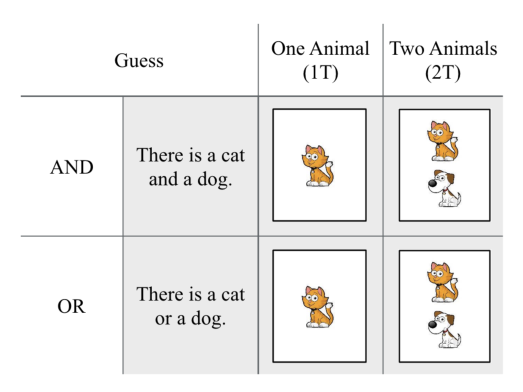
\includegraphics{figs/critical-1} 

}

\caption[Critical trials with example cards]{Critical trials with example cards.}\label{fig:critical}
\end{figure}
\end{CodeChunk}

\subsection{Results}\label{results}

Here we focus on the results of the critical trial types. You can see
the example scenarios of these trial types in Figure 1. These scenarios
include conjunctive and disjunctive guesses with some overlap between
the guessed animals and the animal(s) on the
cards\footnote{Participants judged the trials with no overlap as \textit{wrong} consistently.}.
Figure 2 shows the results for these critical trials. The columns mark
the number of animals on the cards and the rows the type of guess,
namely conjunctive vs.~disjunctive. The number of animals in the
critical trials of this study corresponds to the number of true
conjunct/disjuncts: one animal is 1 conjunct/disjunct true (1T) and two
animals, two conjunct/disjuncts true (2T) (Tieu et al., 2016). Comparing
the rows allows us to know whether adults interpret \emph{and} and
\emph{or} differently. The column comparison shows whether \emph{or} is
interpreted as inclusive or exclusive.

The adult responses differ in both dimensions. First, the response
patterns in the conjunctive and disjunctive trials are different. For
conjunction, the responses are on the extremes of \emph{right} and
\emph{wrong} while for disjunction, they distribute on \emph{kinda
right} and \emph{right}. This pattern suggests that adults interpret
\emph{and} and \emph{or} differently. Second, the responses are
different between the trials where one disjunct/conjuct is true (1T) -
and those that both disjuncts/conjuncts are true (2T). This difference
is greater for conjunction than disjuction. Adults showed a small
preference for the use of disjunction when only one disjunct is true
rather than when both are true. This pattern suggests a small preference
for an exclusive interpretation in the context of this experiment.

\begin{CodeChunk}
\begin{figure}[h]

{\centering 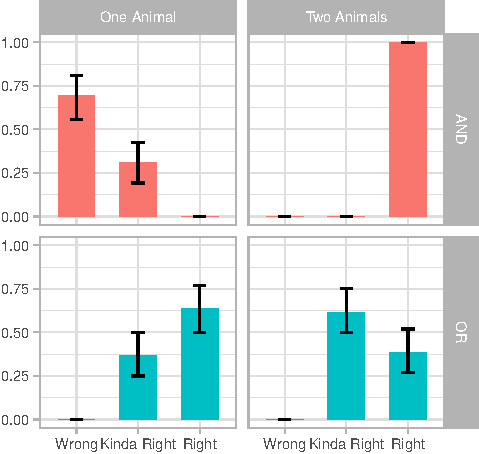
\includegraphics{figs/plot-1} 

}

\caption[Results for Adults' Conjunction and Disjunction Trials]{Results for Adults' Conjunction and Disjunction Trials. Error bars represent 95\% confidence intervals.}\label{fig:plot}
\end{figure}
\end{CodeChunk}

\subsubsection{Individual Responses}\label{individual-responses}

Tieu et al. (2016) and Singh et al. (2016) categorized participants as a
function of their responses to the disjunctive trials. Here we perform a
smiliar analysis on our disjunctive trials. Table 1 summarises the
results. None of the participants considered a disjunctive guess
\emph{wrong} when one or both of the animals were on the card. However,
participants divided into four different groups when interpreting
disjunctive guesses for the one-animal and two-animal scenarios.

The majority of participants (23 out of 52) considered the disjunctive
guess \emph{right} when one animal was on the card (1T), but \emph{kinda
right} with two animals (2T). This pattern is consistent with an
interpretation of ``or'' with an exclusivity implicature. The use of
disjunction when both disjuncts are true is not \emph{wrong} but it is
nevertheless infelicitous and not completely \emph{right}. For these
participants, \emph{kinda right} captures the violation of such a
pragmatic expectation.

The other 29 participants were divided almost equally into the three
remaining groups. 10 participants rated disjunctive guesses as
\emph{right} in both scenarios where one or two animals were on the
card. This pattern is consistent with an inclusive interpretation of
\emph{or} with no exclusivity implicature. 9 other participants rated
disjunctive guesses as only \emph{kinda right} in both one-animal and
two-animal trials. In other words, disjunctive guesses were dispreferred
regardless of the outcome. This response pattern is consistent with the
violation of another pragmatic expectation in the context of a guessing
game: the guesser must choose the most specific guess possible. Under
this expectation, guesses that cover several possible outcomes are
punished. A disjunctive guess never picks a specific outcome and for
these participants, \emph{kinda right} captures the violation of this
specificity expectation.

Finally, 9 participants reported a disjunctive guess as \emph{right}
when both animals were on the card, but only \emph{kinda right} when
only one of the animals was on the card. In other words, these
participants preferred the guess when both disjuncts where true rather
than only one. It is possible that these participants expected a right
guess to be one that brings up a relevant number of animals. When only
one animal is on the card, bringing up a second animal violates this
expectation. When two animals are on the card, bringing up both animals
satisfies this expectation even though the right linguistic connective
was not used. For these participants, the choice of the linguistic
connective (\emph{and} vs. \emph{or}) did not play an important role in
their judgements.

If these speculations are on the right track, we expect participants to
show different response profiles based on how they interpret the goal of
the guessing game and ultimately the meaning of \emph{right} in the
context of the guessing game. We will discuss this issue further in the
last section of this paper.

\begin{table}[t]
\centering
\begin{tabular}{rllr}
  \hline
 & Two Animals.OR & One Animal.OR & Counts \\ 
  \hline
1 & Kinda Right & Kinda Right &   9 \\ 
  2 & Kinda Right & Right &  23 \\ 
  3 & Right & Kinda Right &  10 \\ 
  4 & Right & Right &  10 \\ 
   \hline
\end{tabular}
\caption{This table prints across one column.} 
\end{table}

\subsection{Discussion}\label{discussion}

In this study, we tested adult interpretations of the connective words
\emph{and} and \emph{or} in the context of a guessing game. Adult
participants interpreted these words differently and depending on how
many disjuncts/conjuncts were satisfied. Overall, a guess with
\emph{and} was considered right if both conjuncts were true and wrong if
only one was true. A guess with \emph{or} was not wrong in either case,
yet adults were more likely to consider it as right when only one of the
disjuncts was true. Grouping inviduals based on their responses, we also
found that some participants dispreferred disjunctive guesses whether
one or both disjuncts were true, some considered them better when both
disjucts where true, and some others considered them right in either
case.

The results are consistent with the dominent view on the division of
labor between semantics and pragmatics in the interpretation of
connective words. The semantics of \emph{and} is captured by logical
conjunction and \emph{or} by inclusive disjunction. \emph{And} is true
when both conjuncts are true and false when only one is true. \emph{Or}
is true in both cases but not the best option as a connective when both
disjuncts are true. In Experiment 2 we examine preschool children's
interpretation of these connectives in the conext of the same guessing
game.

\section{Experiment 2}\label{experiment-2}

\subsection{Methods}\label{methods-1}

\subsubsection{Participants}\label{participants-1}

We recruited 42 English speaking children from the Bing Nursery School
at Stanford University. Children were between 3;02 and 5;02 years old
(Mean = 4;04).

\subsubsection{Materials and Design}\label{materials-and-design-1}

We used the same set of cards and linguistic stimuli as the ones in
Experiment 1. The study used 8 trial types and 2 trials per trial type
for the total of 16 trials. The trials were balanced to include the same
number of one-animal and two-animal cards, the same number of simple and
connective guesses, and the same number of expected true vs.~false
judgements. However, we made a few changes to make the experiment more
suitable for childrens. Instead of Bob, a puppet named Jazzy played the
guessing game with the children. Jazzy had a sleeping mask on his eyes
during the game. To introduce a three-valued scale, we placed a set of
red circles, small blue stars, and big blue stars in front of the
children. These tokens were used to reward the puppet after each guess.
The use of tokens as rewards proved to be a more successful measure
during piloting than hand gestures or only verbal feedback (e.g.
\emph{Jazzy you were right!}). One experimenter was involved in this
study.

\subsubsection{Procedure}\label{procedure-1}

The experimenter and the puppet interacted with the children before the
study. The experiment was carried out in a quiet room and the sessions
were videotaped. There was a small table and two chairs in the room.
Children sat on one side of the table and the experimenter and the
puppet on the other side facing the child. The groups of circles, small
stars, and big stars were placed in front of the child from left to
right. A deck of six cards was in front of the experimenter. Similar to
the previous study, participants sat through three phases: introduction,
instruction, and test.

The goal of the introduction phase was to show the animal cards to
children and make sure they recognize the animals and know their names.
The experimenter showed the cards to the children and asked them to
label the animals. All children recognized the animals and could label
them as cat, dog, and elephant. In the instruction phase, children went
through three example trials. The experimenter explained that he is
going to play with the puppet first so that the child can learn the
game. He removed the six introduction cards and placed a deck of three
cards face-down on the table. From top to bottom (first to last), the
cards had the following images: a cat, an elephant, a cat and a dog. He
put the sleeping mask on Jazzy's eyes and explained that Jazzy is going
to guess what is on these cards. He then picked the first card and asked
the puppet: ``\emph{What do you think is on this card?}'' Jazzy replied
with ``\emph{There is a dog}''. The experimenter showed the cat-card to
the child and explained that when Jazzy is \emph{not right} he gets a
circle. He then asked the child to give the puppet a circle. Rewards
were collected by the experimenter and placed under the table to not
distract the child. The second trial followed the same pattern except
that the puppet guessed \emph{right} and the experimenter invited the
child to give the puppet a big star. In the final trial, the puppet
guessed that there is a cat on the card when the card had a cat and a
dog on it. The experimenter said that the puppet was \emph{a little
right} and asked the child to give him a little star.

In the test phase, the experimenter removed the three instruction cards
and placed a deck of 16 randomized cards on the
table\footnote{The randomization code can be found in the github repository of this study}.
The experimenter explained that it is the child's turn to play with the
puppet. The test phase followed the pattern described in the instruction
phase.

\subsubsection{Measurement}\label{measurement-1}

In each trial, children were asked to give the puppet a circle if he is
\emph{wrong}, a small star if he is \emph{a little right}, and a big
star if he is \emph{right}. During the analysis of the videos,
children's linguistic feedback to the puppet after each guess were
categorized into four types: 1. None, 2. Judgements, 3. Descriptions,
and 4. Corrections. The first category referred to cases where children
did not provide any linguistic feedback. Judgements referred to
linguistic feedback such as \emph{you are right!}, \emph{yes},
\emph{nope}, \emph{you winned}. Such feedback only expressed judgements
and mirrored the rewards. Descriptions were cases that the child simply
mentioned what was on the card: \emph{cat!}, \emph{dog and elephant!},
\emph{There is a cat and a dog!} etc. Finally, corrections referred to
feedback that provided corrections to what the puppet had said. Examples
include: \emph{Just a cat!}, \emph{Both!}, \emph{The two are!},
\emph{Only cat}, \emph{cat AND dog} (with emphasis placed on
\emph{and}).

\begin{CodeChunk}
\begin{figure}[h]

{\centering 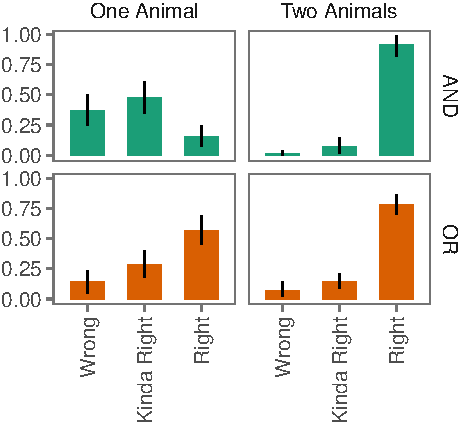
\includegraphics{figs/child_data-1} 

}

\caption[Results for Children's Conjunction and Disjunction Trials]{Results for Children's Conjunction and Disjunction Trials. Error bars represent 95\% confidence intervals.}\label{fig:child_data}
\end{figure}
\end{CodeChunk}

\subsection{Results}\label{results-1}

Figure 3 shows the results. Similar to Experiment 1, comparison of the
rows lets us know whether children differentiate \emph{and} and
\emph{or}. Comparison of the columns in the disjunctive guesses informs
us of exclusivity implicatures. Comparing the conjunction and
disjunction trials (the figure rows), we see that children distinguish
between \emph{and} and \emph{or} in cases where one animal is on the
card but not when both are. Given that the one-animal cojunction trials
(top left) and the one-animal disjunction trials (bottom left) differ in
truth conditions, the difference in response patterns suggests that
children at this age have a different semantic knowledge for \emph{and}
and \emph{or}. The two-animal conjunction and two-animal disjunction
trials (top right and bottom right) do not differ in truth values, and
the responses also show no difference.

In the one-animal and two-animal trials (figure columns), children show
different response patterns when the guess contains the conjunction word
\emph{and} (top right vs.~top left) but not when \emph{or} is used
(bottom right vs.~bottom left). Since the truth values of one-animal and
two-animal trials differ for conjunctive guesses but not disjuncitive
ones, the results suggest that children have different semantic
knowledge for \emph{and} and \emph{or}. The similarity of the
disjunctive guesses in one-animal and two-animal trials (bottom right
vs.~bottom left) can be interpreted as a lack of exclusivity
implicatures in children. We will bring up a caveat to this
interpretationin our analysis of children's linguistic feedback.

Figure 4 shows a side-by-side comparision of adults and children's
responses to the guessing game. We see that adults and children mostly
differ in their interpretation of disjunction when both disjuncts are
true. We also see a difference in one-animal conjunctions trials (top
left) where children show more \emph{kinda right} judgments and fewer
\emph{wrong} ones than adults. We believe that this is due to children's
general reluctance to judge the puppet's guess as \emph{wrong}.

\begin{CodeChunk}
\begin{figure}[h]

{\centering 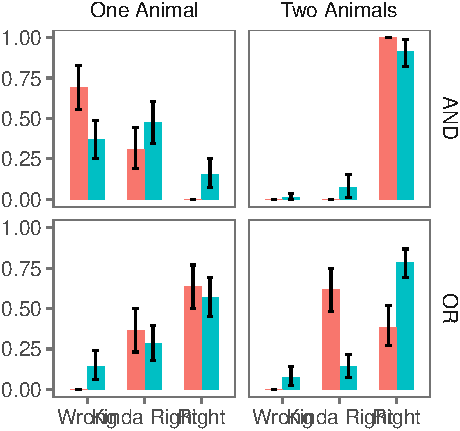
\includegraphics{figs/child_adult_data-1} 

}

\caption[Results for Adults' and Children's Conjunction and Disjunction Trials]{Results for Adults' and Children's Conjunction and Disjunction Trials. Error bars represent 95\% confidence intervals.}\label{fig:child_adult_data}
\end{figure}
\end{CodeChunk}

\subsubsection{Individual Responses}\label{individual-responses-1}

We searched for children that had the following response patterns: they
responded with \emph{wrong} when one disjunct was true but \emph{kinda
right} or \emph{right} when both were true; as well as children that
responded with \emph{kinda right} when one disjuncts was true but
\emph{right} when both were true. We found 10 children with such
response patterns. In Experiment 1 we found similar number of adults
that showed some preference for a disjunctive guess when both disjuncts
were true.

\subsubsection{Linguistic Feedback}\label{linguistic-feedback}

We also categorized children's linguistic feedback to the puppet. Figure
5 shows the results. We excluded the \emph{None} feedback (e.i. the
child did not say anything) since a similar rate of such responses was
present in each trial type. Children's linguistic feedback fell into
three patterns: 1. the one-animal conjunctive and two-animal disjunctive
(top left and bottom right) trials show higher proportion of
\emph{Corrections} than the other trial types. These are trials that the
guesses are either false or infelicitous. The higher number of
corrective feedback in these two trial types hints at children's
sensitivity to both semantic and pragmatic violations. 2. The one-animal
disjunctive trials (bottom left) showed the highest proportion of
\emph{Descriptions}. These are trials that the guess is correct but not
specific enough; leaves two possibilities open. 3. The two-animal
conjunctive trials (top right) show the highest proportion of
\emph{Judgements} such as \emph{you are right!}. This is not surprising
given that in these trials represent the most optimal guessing scenario.

Our analysis of children's linguistic feedback in the context of the
guessing game suggests that children are sensitive to the pragmatics of
the game. More specifically, they produce more corrections to the
puppet's disjunctive guess when both disjuncts are true. Such feedback
suggests that children are sensitive to the exclusivity implicature that
the use of \emph{or} carries. The comparison of children's rewards to
the puppet in the truth value judgment task and their linguistic
feedback raises an important methodological issue. Truth value judgment
tasks alone may not be sufficient for assessing children's pragmatic
competence. In general discussion, we discuss how we intend to address
this issue in our future work.

\begin{CodeChunk}
\begin{figure}[h]

{\centering 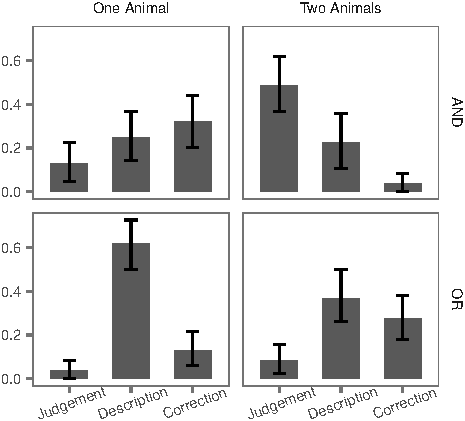
\includegraphics{figs/feedback_data-1} 

}

\caption[Children's Linguistic Feedback to Conjunction and Disjunction Trials]{Children's Linguistic Feedback to Conjunction and Disjunction Trials. Error bars represent 95\% confidence intervals.}\label{fig:feedback_data}
\end{figure}
\end{CodeChunk}

\subsection{Discussion}\label{discussion-1}

This study did not find any evidence for the hypothesis that a large
group of children interpret the disjunction word \emph{or} similar to
its conjunctive counterpart \emph{and}. To the countrary, both
children's judgements and their linguistic feedback suggested that they
differentiate these two connective words. More specifically, children's
jugements mirrored those of adults in conditions with different truth
values. We took this as a sign of children's adult like semantics for
\emph{and} and \emph{or}. However, children's judgements differed from
adults in disjunctive guesses when both disjuncts were true. Children
showed no signs of an exclusivity implicature in such trials. These
results can be interpreted to show that children differ from adults in
the pragmatics of disjunction words.

The analysis of children's linguistic feedback points to a different
possible interpretation of the results. Perhaps children do compute an
exclusivity implicature at the adult rate but they express it
differently. Adults choose to reflect the presence of the implicature in
their judgements while children choose to give corrective linguistic
feedback. In fact, adults in Experiment 1 had no way of offering
linguistic feedback to the guessing character. Had they been able to, it
is possible that they would have shown similar judgment responses to
children.

\section{General Discussion}\label{general-discussion}

We started our investigations with two questions: first, do adults and
more importantly children interpret \emph{and} and \emph{or}
differently? Second, do they interpret \emph{or} as inclusive
disjunction or exclusive disjunciton? In this paper, we presented two
experimental studies to address these questions. Experiment 1 showed
that adults interpreted \emph{or} as a disjunction and differentiated it
from \emph{and}. Judgements of \emph{or} were split between an inclusive
and exclusive interpretation, with a slight advantage for the exclusive
interpretation. Experiment 2 showed that three-to-five-year old children
showed very similar patterns of interpretation in the guessing game
excpet for disjunction when both disjuncts are true. Overall, children
were more likely to interpret \emph{or} as inclusive disjunction.
Therefore, the results of our truth value judgement studies suggest that
both adults and children differentiate \emph{and} and \emph{or}. Yet,
adults are more likely to interpret \emph{or} as exclusive while
children interpret it as inclusive. These results are most compatible
with the ones reported in Crain (2012).

At this point, we would like to discuss two issues raised by Experiments
1 and 2 that we would like to address in the future. First, the analysis
of individual adult responses in experiment 1 showed that adults
interpret \emph{or} in many different ways, even though the majority
stick to an exclusive interpretion. We suspect that this variation is
due to participants' understanding of the goal of the game and
ultimately what being \emph{right} means in the context of the game. If
this hypothesis is true, it should be possible to experimentally
manipulate the goal of the game and assess the change in adult
interpretations of \emph{or}.

Second, in our analysis of children's linguistic feedback we saw signs
of children's sensitivity to exclusivity implicatures that were not
captured by the standard truth value judgement task. These results
suggest that truth value judgement tasks may not be sufficient in
assessing children's pragmatic competence and should be supplemented
with other assessments such as elicitation of linguistic feedback to
pragmatically infelicitious utterances. We would like to pursue this
line of research in future work.

\section{Acknowledgements}\label{acknowledgements}

We would like to thank Eve V. Clark and Christopher Potts for their
generous help and advice on this project. We would also like to thank
the staff and children at Stanford's Bing Nursery School. This work was
supported by NSF \#1456077.

\section{References}\label{references}

\setlength{\parindent}{-0.1in} \setlength{\leftskip}{0.125in} \noindent

\hypertarget{refs}{}
\hypertarget{ref-braine1981development}{}
Braine, M. D., \& Rumain, B. (1981). Development of comprehension of
``or'': Evidence for a sequence of competencies. \emph{Journal of
Experimental Child Psychology}, \emph{31}(1), 46--70.

\hypertarget{ref-chierchia2001acquisition}{}
Chierchia, G., Crain, S., Guasti, M. T., Gualmini, A., \& Meroni, L.
(2001). The acquisition of disjunction: Evidence for a grammatical view
of scalar implicatures. In \emph{Proceedings of the 25th boston
university conference on language development} (pp. 157--168).
Cascadilla Press Somerville, MA.

\hypertarget{ref-crain2008interpretation}{}
Crain, S. (2008). The interpretation of disjunction in universal
grammar. \emph{Language and Speech}, \emph{51}(1-2), 151--169.

\hypertarget{ref-crain2012emergence}{}
Crain, S. (2012). \emph{The emergence of meaning}. Cambridge University
Press.

\hypertarget{ref-crain1998investigations}{}
Crain, S., \& Thornton, R. (1998). \emph{Investigations in universal
grammar: A guide to experiments on the acquisition of syntax and
semantics}. MIT Press.

\hypertarget{ref-grice1975logicconvo}{}
Grice, H. P. (1975). Logic and conversation. In P. Cole \& J. Morgan
(Eds.), \emph{Syntax and semantics} (Vol. 3: Speech Acts, pp. 43--58).
Academic Press.

\hypertarget{ref-johansson1975preschool}{}
Johansson, B. S., \& Sjölin, B. (1975). Preschool children's
understanding of the coordinators ``and'' and ``or''. \emph{Journal of
Experimental Child Psychology}, \emph{19}(2), 233--240.

\hypertarget{ref-katsos2011pragmatic}{}
Katsos, N., \& Bishop, D. V. (2011). Pragmatic tolerance: Implications
for the acquisition of informativeness and implicature.
\emph{Cognition}, \emph{120}(1), 67--81.

\hypertarget{ref-notley2012children}{}
Notley, A., Zhou, P., Jensen, B., \& Crain, S. (2012). Children's
interpretation of disjunction in the scope of ``before'': A comparison
of english and mandarin. \emph{Journal of Child Language},
\emph{39}(03), 482--522.

\hypertarget{ref-Singh2016}{}
Singh, R., Wexler, K., Astle-Rahim, A., Kamawar, D., \& Fox, D. (2016).
Children interpret disjunction as conjunction: Consequences for theories
of implicature and child development. \emph{Natural Language Semantics},
\emph{24}(4), 305--352. \url{http://doi.org/10.1007/s11050-016-9126-3}

\hypertarget{ref-tieu2016}{}
Tieu, L., Yatsushiro, K., Cremers, A., Romoli, J., Sauerland, U., \&
Chemla, E. (2016). On the role of alternatives in the acquisition of
simple and complex disjunctions in french and japanese. \emph{Journal of
Semantics}.

\end{document}
